\documentclass{article}
\usepackage[margin = 0.3in]{geometry}
\usepackage{amsfonts, setspace, graphicx, amsmath, bbm}
\graphicspath{{./images/}}
\begin{document}
    \onehalfspacing

    \begin{singlespace}
        \title{CSE 417T: Homework 2} 
        \author{Hangxiao Zhu}
        \date{\today}
        \maketitle
    \end{singlespace}

    \section*{Problem 1.}
    a. Report on each of the maximum number of iterations:
    \begin{center}
        \begin{tabular}{|c|c|c|c|c|c|}
            \hline
            Maximum Iterations & Training time & Iterations & $E_{in}$ & $e$ on training set & $e$ on test set\\
            \hline
            10000 & 0.07678604125976562 & 10000 & 0.5847165561996043 & 0.3092105263157895 & 0.31724137931034485\\
            \hline
            100000 & 0.7698559761047363 & 100000 & 0.4937022212468817 & 0.2236842105263158 & 0.20689655172413793\\
            \hline
            1000000 & 7.694957971572876 & 1000000 & 0.43535262292978577 & 0.1513157894736842 & 0.1310344827586207\\
            \hline
        \end{tabular}
    \end{center}
    Based on the binary classification errors in the training and test, the model performs no worse in the test set 
    than in the training set. That means the generalization properties of the model is very strong.\\
    By increasing the maximum number of iterastions, the binary classification errors on test data gradually decreases, 
    that is, the model's performance gets improved by increasing the number of training iterations.\\
    b. I normalized both datasets using the training mean and variance.\\
    The mean I used is [54.5855263, 0.657894737, 3.125, 130.532895, 249.835526, 0.131578947, 
    0.914473684, 149.565789, 0.269736842, 1.00263158, 1.57894737, 0.651315789, 4.80263158].\\
    The variance I used is [78.8084747, 0.225069252, 0.938322368, 315.735760, 3199.82163, 0.114265928, 0.986106302, 
    550.258830, 0.196978878, 1.17551939, 0.362188366, 0.819208795, 3.76367729].\\
    The standard deviation I used is [8.87741374, 0.47441464, 0.96867041, 17.76895495, 56.56696591, 0.33803244, 
    0.99302885,\\ 23.45759642, 0.44382303, 1.08421372, 0.60182088, 0.90510154, 1.94001992].\\
    Report on each of the learning rate:
    \begin{center}
        \begin{tabular}{|c|c|c|c|c|c|}
            \hline
            $\eta$ & Training time & Iterations & $E_{in}$ & $e$ on training set & $e$ on test set\\
            \hline
            0.01 & 7.577642917633057 & 1000000 & 0.4073814412083029 & 0.17105263157894737 & 0.1103448275862069\\
            \hline
            0.1 & 7.762326002120972 & 1000000 & 0.4073814412083028 & 0.17105263157894737 & 0.1103448275862069\\
            \hline
            1 & 0.006412029266357422 & 819 & 0.40738144120830283 & 0.17105263157894737 & 0.1103448275862069\\
            \hline
            4 & 0.0015261173248291016 & 186 & 0.40738144120830283 & 0.17105263157894737 & 0.1103448275862069\\
            \hline
            7 & 0.001306772232055664 & 164 & 0.40738144120830283 & 0.17105263157894737 & 0.1103448275862069\\
            \hline
            7.5 & 0.005311012268066406 & 678 & 0.40738144120830294 & 0.17105263157894737 & 0.1103448275862069\\
            \hline
            7.6 & 0.023669004440307617 & 3051 & 0.40738144120830283 & 0.17105263157894737 & 0.1103448275862069\\
            \hline
            7.7 & 8.204280138015747 & 1000000 & 0.40843667430393826 & 0.16447368421052633 & 0.11724137931034483\\
            \hline
        \end{tabular}
    \end{center}
    Normalizing the data did affect the performace of the model. By observing the table above, we can see the 
    cross-entropy error on the training data set, the binary classification error on both the training and test data 
    sets all decreases after normalizing the data. Thus, I think normalizing the data boost the performace of the 
    model.\\
    Changing learning rate $\eta$ affects the number of iterations the gradient descent takes to converge. Choosing 
    a proper learning rate can significantly improve the efficiency of the model and reduce the number of iterations 
    required to converge. However, if the learning rate is too small or too large, the number of iterations required 
    to converge will be large.

    \section*{Problem 2.}
    Based on $E_{out}(g^{(\mathcal{D})}) = \mathbb{E}_{\mathbf{x},y}[(g^{(\mathcal{D})}(\mathbf{x}) - y(x))^2]$ and 
    $y(x) = f(x) + \epsilon$, we can deduce that:
    \begin{align*} 
        \mathbb{E}_{\mathcal{D}}[E_{out}(g^{(\mathcal{D})})] & = 
        \mathbb{E}_{\mathcal{D}}[\mathbb{E}_{\mathbf{x},y}[(g^{(\mathcal{D})}(\mathbf{x}) - y(x))^2]]\\
        & = \mathbb{E}_{\mathbf{x},y}[\mathbb{E}_{\mathcal{D}}
        [(g^{(\mathcal{D})}(\mathbf{x}) - \bar{g}(\mathbf{x}) + \bar{g}(\mathbf{x}) - y(x))^2]]\\
        & = \mathbb{E}_{\mathbf{x},y}[\mathbb{E}_{\mathcal{D}}
        [(g^{(\mathcal{D})}(\mathbf{x}) - \bar{g}(\mathbf{x}))^2 + (\bar{g}(\mathbf{x}) - y(x))^2
        + 2(g^{(\mathcal{D})}(\mathbf{x}) - \bar{g}(\mathbf{x}))(\bar{g}(\mathbf{x}) - y(x))]]\\
        & (Note \ that \ 
        \mathbb{E}_{\mathcal{D}}[(g^{(\mathcal{D})}(\mathbf{x}) - \bar{g}(\mathbf{x}))(\bar{g}(\mathbf{x}) - y(x))] 
        = (\bar{g}(\mathbf{x}) - y(x))\mathbb{E}_{\mathcal{D}}[(g^{(\mathcal{D})}(\mathbf{x}) - \bar{g}(\mathbf{x}))] 
        = 0)\\
        & = \mathbb{E}_{\mathbf{x},y}[\mathbb{E}_{\mathcal{D}}
        [(g^{(\mathcal{D})}(\mathbf{x}) - \bar{g}(\mathbf{x}))^2 + (\bar{g}(\mathbf{x}) - y(x))^2]]\\
        & = \mathbb{E}_{\mathbf{x},y}[\mathbb{E}_{\mathcal{D}}
        [(g^{(\mathcal{D})}(\mathbf{x}) - \bar{g}(\mathbf{x}))^2]] + 
        \mathbb{E}_{\mathbf{x},y}[(\bar{g}(\mathbf{x}) - y(x))^2]\\
        & = \mathbb{E}_{\mathbf{x},y}[Variance \ of \ g^{(\mathcal{D})}(\mathbf{x})] + 
        \mathbb{E}_{\mathbf{x},y}[(\bar{g}(\mathbf{x}) - f(x) - \epsilon)^2]\\
        & = \mathbb{E}_{\mathbf{x},y}[Variance \ of \ g^{(\mathcal{D})}(\mathbf{x})] + 
        \mathbb{E}_{\mathbf{x},y}[(\bar{g}(\mathbf{x}) - f(x))^2 - 2(\bar{g}(\mathbf{x}) - f(x))\epsilon 
        + \epsilon^2]\\
        & = \mathbb{E}_{\mathbf{x},y}[Variance \ of \ g^{(\mathcal{D})}(\mathbf{x})] + 
        \mathbb{E}_{\mathbf{x},y}[(\bar{g}(\mathbf{x}) - f(x))^2] + \mathbb{E}_{\mathbf{x},y}[\epsilon^2] - 
        2\mathbb{E}_{\mathbf{x},y}[(\bar{g}(\mathbf{x}) - f(x))\epsilon]\\
        & = \mathbb{E}_{\mathbf{x}}[Variance \ of \ g^{(\mathcal{D})}(\mathbf{x})] + 
        \mathbb{E}_{\mathbf{x}}[Bias \ of \ \bar{g}(\mathbf{x})] + \mathbb{E}_{\mathbf{x},y}[\epsilon^2] - 
        2\mathbb{E}_{\mathbf{x},y}[(\bar{g}(\mathbf{x}) - f(x))\epsilon]\\
        & = var + bias + \mathbb{E}_{\mathbf{x},y}[\epsilon^2] - 
        2\mathbb{E}_{\mathbf{x},y}[(\bar{g}(\mathbf{x}) - f(x))\epsilon]\\
        & = var + bias + \mathbb{E}_{\epsilon}[\epsilon^2] - 
        2\mathbb{E}_{\mathbf{x}}[(\bar{g}(\mathbf{x}) - f(x))\epsilon]\\
        & = var + bias + \mathbb{E}_{\epsilon}[\epsilon^2] - 
        2\mathbb{E}_{\mathbf{x}}[(\bar{g}(\mathbf{x}) - f(x))]\mathbb{E}_{\mathbf{x}}[\epsilon]\\
        & = var + bias + \mathbb{E}_{\epsilon}[\epsilon^2] - 
        2\mathbb{E}_{\mathbf{x}}[(\bar{g}(\mathbf{x}) - f(x))]\mathbb{E}_{\epsilon}[\epsilon]\\
        & (Note \ that \ \epsilon is \ a \ zero \ mean \ noise, \ which \ means \  \bar{\epsilon} = 
        \mathbb{E}_{\epsilon}[\epsilon] = 0)\\
        & = var + bias + \mathbb{E}_{\epsilon}[(\epsilon - \bar{\epsilon})^2]\\
        & = var + bias + \sigma^2\\
        & = \sigma^2 + bias + var
    \end{align*}

    \section*{Problem 3.}
    (a) Since the input variable $x$ is uniformly distributed in the interval $[-1, 1]$, we know 
    $\bar{x} = \mathbb{E}_{\mathbf{D}}[x] = 0$. Based on them, we can deduce that:
    \begin{align*}
        \bar{g}(x) & = \mathbb{E}_{\mathbf{D}}[g(x)]\\
        & = \mathbb{E}_{\mathbf{D}}[ax + b]\\
        & (Note \ that \ a = \frac{x_2^2 - x_1^2}{x_2 - x_1} = x_1 + x_2, 
        \ b = \frac{x_1x_2^2 - x_2x_1^2}{x_2 - x_1} = -x_1x_2)\\
        & = \mathbb{E}_{\mathbf{D}}[(x_1 + x_2)x - x_1x_2]\\
        & = (\mathbb{E}_{\mathbf{D}}[x_1] + \mathbb{E}_{\mathbf{D}}[x_2])x - 
        \mathbb{E}_{\mathbf{D}}[x_1]\mathbb{E}_{\mathbf{D}}[x_2]\\
        & = 0
    \end{align*}
    (b) Experiment to determine $\bar{g}(x)$:
    \begin{itemize}
        \item Sample a $x$ from the interval $[-1, 1]$ according to uniform distribution.
        \item Iterate t times (i.g. t = 1000):
        \begin{itemize}
            \item Sample two datapoints uniformly from the interval $[-1, 1]$.
            \item Compute $a$ and $b$.
            \item Compute the value of $g^{(\mathcal{D})}(x)$ and save the result in an array.
        \end{itemize}
        \item Compute $\bar{g}(x)$ by taking the average of the array of $g^{(\mathcal{D})}(x)$.
    \end{itemize}
    Experiment to determine $E_{out}, \ bias, \ var$:
    \begin{itemize}
        \item Iterate t times (i.g. t = 10000):
        \begin{itemize}
            \item Sample a $x$ from the interval $[-1, 1]$ according to uniform distribution.
            \item Follow the experiment described above to calculate the array of $g^{(\mathcal{D})}(x)$ 
            and $\bar{g}(x)$. 
            \item Use $\mathbb{E}_{\mathcal{D}}[(g^{(\mathcal{D})}(\mathbf{x}) - \bar{g}(\mathbf{x}))^2]$ to 
            calculate $var$ and save the result in an array.
            \item Use $(\bar{g}(\mathbf{x} - f(\mathbf{x}))^2$ to calculate $bias$ and save the result in an array.
            \item Use $\mathbb{E}_{\mathcal{D}}[(g^{(\mathcal{D})}(\mathbf{x}) - f(\mathbf{x}))^2]$ to calculate
            $E_{out}$ and save the result in an array.
        \end{itemize}
        \item Compute $E_{out}, \ bias, \ var$ by taking the average of the arrays of $E_{out}, \ bias, \ var$.
    \end{itemize}
    (c) As shown in the table below, $E_{out} \approx bias + var$, which is consistent with the theoretical result.
    \begin{center}
        \begin{tabular}{|c|c|c|c|}
            \hline
            $E_{out}$ & $bias$ & $var$ & $bias + var$\\
            \hline
            0.5430268888689767 & 0.2051878468504339 & 0.33732433111079485 & 0.5425121779612287\\
            \hline
        \end{tabular}
    \end{center}   
    \begin{figure}[!htb]
        \begin{center}
            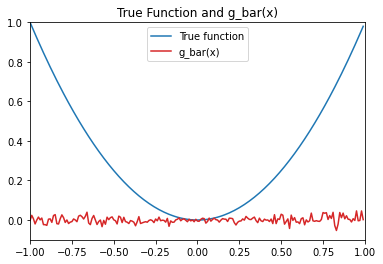
\includegraphics[width=10cm, height=8cm]{gxfx.png}
            \textbf{\caption{Histogram of Number of Iterations}}
        \end{center}
    \end{figure}
    (d) Calculate $bias$:
    \begin{align*} 
        bias & = \mathbb{E}_{\mathbf{x}}[(\bar{g}(\mathbf{x} - f(\mathbf{x}))^2]\\
        & = \mathbb{E}_{\mathbf{x}}[f(\mathbf{x})^2]\\
        & = \mathbb{E}_{\mathbf{x}}[(\mathbf{x}^2)^2]\\
        & = \mathbb{E}_{\mathbf{x}}[\mathbf{x}^4]\\
        & = \frac{1}{2}\int_{-1}^{1} x^4 dx\\
        & = \frac{1}{5}
    \end{align*}

    Calculate $var$:
    \begin{align*} 
        var & = \mathbb{E}_{\mathbf{x}}[\mathbb{E}_{\mathcal{D}}[(g^{(\mathcal{D})}(\mathbf{x}) - 
        \bar{g}(\mathbf{x}))^2]]\\
        & = \mathbb{E}_{\mathbf{x}}[\mathbb{E}_{\mathcal{D}}[(a\mathbf{x}+b)^2]]\\
        & (Note \ that \ a = \frac{x_2^2 - x_1^2}{x_2 - x_1} = x_1 + x_2, 
        \ b = \frac{x_1x_2^2 - x_2x_1^2}{x_2 - x_1} = -x_1x_2)\\
        & = \mathbb{E}_{\mathbf{x}}[\mathbb{E}_{\mathcal{D}}[(x_1 + x_2)^2\mathbf{x}^2 + x_1^2x_2^2 - 
        2x_1x_2(x_1 + x_2)\mathbf{x}]]\\
        & = \mathbb{E}_{\mathbf{x}}[\mathbb{E}_{\mathcal{D}}[x_1^2 + x_2^2 + 2x_1x_2]\mathbf{x}^2 + 
        \mathbb{E}_{\mathcal{D}}[x_1^2x_2^2] - 2\mathbb{E}_{\mathcal{D}}[x_1^2x_2 + x_2^2x_1]\mathbf{x}]\\
        & = \mathbb{E}_{\mathbf{x}}[(\mathbb{E}_{\mathcal{D}}[x_1^2] + \mathbb{E}_{\mathcal{D}}[x_2^2] +
        2\mathbb{E}_{\mathcal{D}}[x_1x_2])\mathbf{x}^2 + 
        \mathbb{E}_{\mathcal{D}}[x_1^2]\mathbb{E}_{\mathcal{D}}[x_2^2] - 
        2\mathbb{E}_{\mathcal{D}}[x_1x_2]\mathbb{E}_{\mathcal{D}}[x_1 + x_2]\mathbf{x}]\\
        & (Note \ that \ \mathbb{E}_{\mathcal{D}}[x^2] = \frac{1}{2}\int_{-1}^{1} x^2 dx = \frac{1}{3},
        \mathbb{E}_{\mathcal{D}}[x_1x_2] = 0)\\
        & = \mathbb{E}_{\mathbf{x}}[\frac{2}{3}\mathbf{x}^2 + \frac{1}{9}]\\
        & = \frac{2}{3}\mathbb{E}_{\mathbf{x}}[\mathbf{x}^2] + \frac{1}{9}\\
        & = \frac{2}{3} \times \frac{1}{3} + \frac{1}{9}\\
        & = \frac{1}{3}
    \end{align*}

    Calculate $E_{out}$:
    \begin{align*} 
        \mathbb{E}_{\mathcal{D}}[E_{out}(g^{(\mathcal{D})})] & = 
        \mathbb{E}_{\mathcal{D}}[\mathbb{E}_{out}[(g^{(\mathcal{D})}(\mathbf{x}) - y(x))^2]]\\
        & = bias + var\\
        & = \frac{1}{5} + \frac{1}{3}\\
        & = \frac{8}{15}
    \end{align*}

    \section*{Problem 4.}
    (a) We can write $E_n(\mathbf{w})$ as 
    \begin{align*} 
        E_n(\mathbf{w}) = 
            \begin{cases}
                0 & y_n\mathbf{w}^T\mathbf{x}_n \geq 1\\
                (1 - y_n\mathbf{w}^T\mathbf{x}_n)^2 & y_n\mathbf{w}^T\mathbf{x}_n < 1
            \end{cases}
    \end{align*}
    We can see that when $y_n\mathbf{w}^T\mathbf{x}_n > 1$, $E_n(\mathbf{w}) = 0$ is continuous and differentiable, 
    when $y_n\mathbf{w}^T\mathbf{x}_n \to 1$, $E_n(\mathbf{w}) = 0$, when $y_n\mathbf{w}^T\mathbf{x}_n < 1$, 
    $E_n(\mathbf{w}) = (1 - y_n\mathbf{w}^T\mathbf{x}_n)^2$ is continuous and differentiable.\\
    The gradient $\nabla E_n(\mathbf{w})$ is
    \begin{align*} 
        \nabla E_n(\mathbf{w}) = 
            \begin{cases}
                0 & y_n\mathbf{w}^T\mathbf{x}_n \geq 1\\
                -2y_nx_n(1 - y_n\mathbf{w}^T\mathbf{x}_n) & y_n\mathbf{w}^T\mathbf{x}_n < 1
            \end{cases}
    \end{align*}
    (b) I will prove by two cases:\\
    \textbf{Case 1:} If $sign(\mathbf{w}^T\mathbf{x}_n) \neq y_n$, then 
    $\mathbbm{1}[sign(\mathbf{w}^T\mathbf{x}_n) \neq y_n] = 1$ and $y_n\mathbf{w}^T\mathbf{x}_n \leq 0$. Therefore, 
    $E_n(\mathbf{w}) = (1 - y_n\mathbf{w}^T\mathbf{x}_n)^2 \geq 1$. Thus, $E_n(\mathbf{w}) \geq 
    \mathbbm{1}[sign(\mathbf{w}^T\mathbf{x}_n) \neq y_n]$.\\
    \textbf{Case 2:} If $sign(\mathbf{w}^T\mathbf{x}_n) = y_n$, then
    $\mathbbm{1}[sign(\mathbf{w}^T\mathbf{x}_n) \neq y_n] = 0$ and $y_n\mathbf{w}^T\mathbf{x}_n \geq 0$. Therefore, 
    when $0 \leq y_n\mathbf{w}^T\mathbf{x}_n < 1$, $E_n(\mathbf{w}) = (1 - y_n\mathbf{w}^T\mathbf{x}_n)^2 \geq 0$, 
    when $y_n\mathbf{w}^T\mathbf{x}_n \geq 1$, $E_n(\mathbf{w}) = 0$. In both situations, $E_n(\mathbf{w}) \geq 
    \mathbbm{1}[sign(\mathbf{w}^T\mathbf{x}_n) \neq y_n]$.\\
    In conclusion, $E_n(\mathbf{w}) \geq \mathbbm{1}[sign(\mathbf{w}^T\mathbf{x}_n) \neq y_n]$, which means 
    $E_n(\mathbf{w})$ is an upper bound for $\mathbbm{1}[sign(\mathbf{w}^T\mathbf{x}_n) \neq y_n]$. Hence, 
    $\frac{1}{N}\sum_{n=1}^{N}E_n(\mathbf{w})$ is an upper bound for $E_{in}(\mathbf{w})$.\\
    (c) The stochastic gradient descent should be in the following steps:
    \begin{itemize}
        \item Initialize a $\mathbf{w}$. 
        \item Iterate t times:
        \begin{itemize}
            \item Randomly choose $x_n, y_n$.
            \item Let $s_t = \mathbf{w}^T\mathbf{x}_n$, then $y_ns_t = y_n\mathbf{w}^T\mathbf{x}_n$.
            \item If $y_n\mathbf{w}^T\mathbf{x}_n \geq 1$, $\nabla E_n(\mathbf{w}) = 0$, then 
            $w \gets w - \eta\nabla E_n(\mathbf{w}) = w - 0 = w$.
            \item If $y_n\mathbf{w}^T\mathbf{x}_n < 1$, $\nabla E_n(\mathbf{w}) = 
            -2y_nx_n(1 - y_n\mathbf{w}^T\mathbf{x}_n)$, then $w \gets w - \eta\nabla E_n(\mathbf{w}) = 
            w + 2\eta y_nx_n(1 - y_ns_t)$. Then replace $2\eta$ by $\eta'$, $w = w + \eta' y_nx_n(1 - y_ns_t)$.
        \end{itemize}
    \end{itemize}
    We can see the process above is the same as the Adaline algorithm, therefore the Adaline algorithm performs
    stochastic gradient descent on $\frac{1}{N}\sum_{n=1}^{N}E_n(\mathbf{w})$.

    \section*{Problem 5.}
    (a) This transformation $\Phi(\mathbf{x})$ converts each data point into $N$ dimension, although PLA has
    $d_{vc} = N + 1$, it is still very expensive to compute on this dataset. Besides, since the $d_{vc} = N + 1$, 
    this hypothesis has a very large $d_{vc}$, which makes it hard to minimize the generalization error.\\
    (b) This transformation $\phi_n(\mathbf{x})$ requires extra storage for each data which is not in the dataset.
    Therefore, more storage is required.\\
    (c) When $N$ gets large and the original data set has large dimensions, the storage will be significantly large 
    becase each data point will be converted into $101-d$ data. Also, the computation will also be slow since the 
    transformation requires to traverse $i, j$.

\end{document}